\documentclass[border=10pt]{standalone}
\usepackage{pgfplots}
\usepgfplotslibrary{colormaps}
\pgfplotsset{compat=newest}
\begin{document}
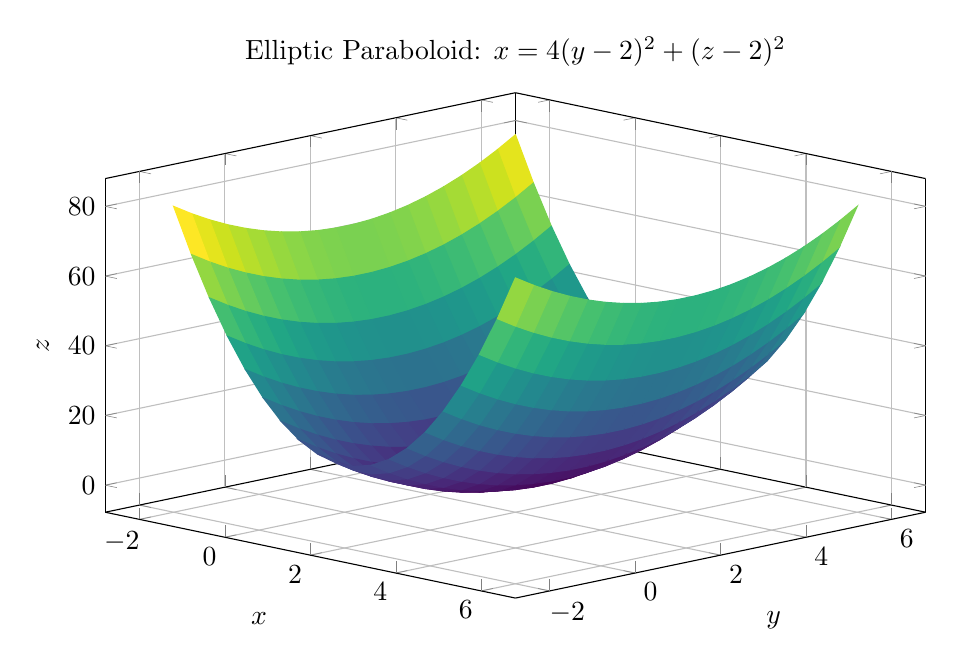
\begin{tikzpicture}
\begin{axis}[
    view={45}{20},
    xlabel={$x$},
    ylabel={$y$},
    zlabel={$z$},
    title={Elliptic Paraboloid: $x = 4(y-2)^2 + (z-2)^2$},
    colormap/viridis,
    samples=20,
    domain=-2:6,
    y domain=-2:6,
    enlargelimits=0.1,
    grid=major,
    width=12cm,
    height=8cm
]
\addplot3[surf, shader=flat corner] 
    {4*(x-2)^2 + (y-2)^2};
\end{axis}
\end{tikzpicture}
\end{document}
